\documentclass[a4paper, 12pt]{article}
\usepackage[english, russian]{babel} % для русского языка
\usepackage[utf8]{inputenc}
\usepackage[T2A]{fontenc}
\usepackage{amssymb} 
\usepackage{amsmath}
\usepackage{amsthm} %для Теорем
\usepackage{amsmath}
\usepackage{caption}
\usepackage{indentfirst} %для отступа в первом абзаце
\usepackage{geometry}
\usepackage{titleps}
\usepackage{graphicx}
\usepackage{soulutf8}
\usepackage{booktabs}
\usepackage{textcomp}
\usepackage{gensymb}
\usepackage{array}
\makeatletter

\newcommand{\vkip}[1]{\vspace{#1\baselineskip}}

\author{Александр Ромачевский}
\date{}

\begin{document}
\setcounter{secnumdepth}{0}
\thispagestyle{empty}
\begin{center}
\Huge
\textbf{Лабораторная работа 3.1.1}\newline

Измерение магнитного поля Земли
\vskip 470 pt

\Large\quad \quad \quad Ромачевский А. Б01--404\newline
МФТИ, Долгопрудный 2025
\end{center}
\clearpage
\newpage
\newpage

\section{Введение}

\textbf{Цель работы:}
определить характеристики шарообразных неодимовых
магнитов и, испольщуя составляющие индукции магнитного поля Земли и 
магнитное наклонение.

\textbf{Оборудование:} 12 одинаковых неодимовыхмагнитных шариков, тонкая нить для изготовления крутильного маятника, медная проволока диаметром (0,5-0,6) мм,
электронные весы, сеундомер, измеритель магнитной индукции ATE-8702, штангенциркуль, брусок из немагнитного материала (25Х30Х60 $\text{мм}^3$), деревяная линейка, штатив из немагнитного материала;
дополнительные неодимовые магнитны ешарики (~20 шт.) и неодимовые магниты в форме параллелепипедов (2 шт.), набор гирь и разновесов.

\textbf{Измерительные погрешности:}\newline
Погрешность электронных весов: $\varepsilon_m=0,001$ г\newline
Погрешность измерения времени: $\varepsilon_t=0,6$ с\newline
Погрешность измерения магнитной индукции: $\varepsilon_B=$\newline 

\newpage
\section{1. Теоретические сведения}
\subsection{Основные формулы}
Простейший магнитный диполь может быть образован витком с током или постоянным магнитом. По определению, магнитный момент $m$ тонкого витка площадью $S$ с током $I$ равен $\mathfrak{m} = \frac{I\textbf{S}}{c}, $где $\textbf{S} = S\textbf{n}$ - вектор площади контура, образующий с направлением тока правовинтовую систему, $\textbf{n}$ - единичный вектор нормали к площадке. Если размеры контура с током или магнитной стрелки малы по сравнению с расстоянием до диполя, то соответствующий магнитный диполь называют \textit{элементарным}, или \textit{точечным}.

Магнитное поле точечного диполя определяется по формуле, анологичной формуле для поля элементарного электрического диполя:

\[\textbf{B}_{дип} = \frac{3(\mathfrak{m} \cdot \textbf{r})\textbf{r}}{r^5} - \frac{\textbf{m}}{r^3}\]

Во внешнем магнитном поле с индукцией $\textbf{B}$ на точеный магнитный диполь $\mathfrak{m}$ действует механический момент сил $\textbf{M}=[\mathfrak{m}, \textbf{B}] $
При этом потенциальная энергия которой обладает диполь с постоянным $\mathfrak{m}$, равна
$W = -(\mathfrak{m} \cdot \textbf{B})$
Когда диполь ориентирован вдоль внешнего поля, он находится в состоянии \textit{равновесия}.

В \textit{неоднородном} внешнем поле выражение для энергии постоянного диполя сохраняется. При этом кроме момента сил на диполь действует ещё и сила

\[\textbf{F} = -\nabla W = (\mathfrak{m} \cdot \nabla)\textbf{B}\]

Таким образом из вышесказанного следует, что \textit{свободный} магнитный диполь в неоднородном магнитном поле ориентируется вдоль силовых линий магнитного поля и втягивается в область более сильного поля, поскольку это ведёт к уменьшению энергии диполя.

Выражения выше, позволяют рассчитать силу взаимодействия магнитов с моментами $\mathfrak{m_1}$ и $\mathfrak{m_2}$. Kогда моменты двух небольших магнитов направлены вдоль соединяющей их прямой: $\mathfrak{m_{1,2}} \| \textbf{r}$, где $\textbf{r}$ - радиус-вектор между ними, они взаимодействуют с силой
\[F_{12}= \mathfrak{m_1} \frac{\partial{B_2}}{\partial{r}} = \mathfrak{m_1}\frac{\partial{(2\mathfrak{m_2}/r^3)}}{\partial{r}} = -\frac{6 \mathfrak{m_1}\mathfrak{m_2}}{r^4} \;(\text{ед.\; СГС}) \]


Если магнитные моменты направлены перпендикулярно соединяющей их прямой: $\mathfrak{m_{1,2}} \perp \textbf{r}$, то нетрудно показать, что сила их взаимодействия окажется в два раза меньшей и будет иметь противоположный знак: $$F_{12} = \frac{3\mathfrak{m_1} \mathfrak{m_2}}{r^4}\;(\text{ед. СГС}) $$.


\newpage
\subsection{Экспериментальная установка}

\newpage 

\section{2. Ход работы}
\subsection{Определение магнитного момента, намагниченности и остаточной магнитной
индукции вещества магнитных шариков}
\subsection{Метод А}
Вычсислим характеристики шаров. Взвесим их,
вычислим $r_\text{max}$ - максимальное расстояние, на котором шарики удерживают друг друга в 
поле силы тяжести Земли.
Для этого воспольуземся специальным стэндом (рис.2)\newline
Измерим для 4 пар и усредним. Измерим диаметры шариков.
\begin{figure}[h]
  \centering    
    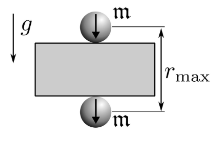
\includegraphics[width=0.5\textwidth]{Images/rmax.png}
    \caption{Стэнд для определения $r_\text{max}$}
\end{figure}

\[r_\text{max}=2,5 \text{ см}\]

Теперь измерим диаметры шариков. Вычислим магнитный момент и намагниченность по формулам, 
затем вычислим их с помощью магнитометра. Результаты измерений занесем в таблицу (Таблица 1).


С помощью магнитометра изерим индукцию на полюсах и получим результат, несколько отличающийся
от полученного теоретически: $B_\text{Avg} = 1950\text{Гс}$. Расхождение небольшое, поэтому
проводить повторные измерения момента не будем.

\newpage
\subsection{Метод B}
Составим цепочку из 20 шарикови и с помощью
неодимовых магнитов в форме параллелепипедов, подсоединим цепочку у к гире и разновесам.

 Добавляя или удаляя шарики, подберем минимальный вес
F системы цепочки с гирей, при котором она отрывается от верхнего шарика:
\begin{figure}[h]
  \centering
  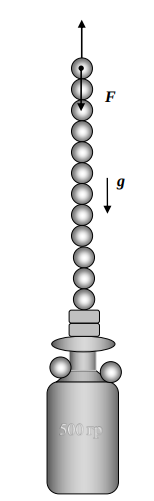
\includegraphics[width=0.1\textwidth]{Images/MethB.png}
  \caption{Определение магнитного момента методом B}
\end{figure} 

Получаем $F=2.3\text{Н}$. $F_0=F/1.08=2.1$Н. Магнитный момент получим из формулы
$P_m=d^2\sqrt{\frac{F_0}{6}}$: $P_m=1983\text{Гс}$ ($\varepsilon_{P_m}=0.04$).

Этот результат совпадает со снятым магнитометром значением, погрешность метода меньше
в 2 раза, поэтому метод B можно считать лучшим способом определения магнитного момента шаров.
\begin{table}[h]
\centering
\begin{tabular}{|c|c|c|c|c|c|c|c|c|c|c|}
\hline
N & m, г & $\varepsilon_m$ & d, см & $\varepsilon_d$ & $P_m$, $\frac{\text{эрг}}{\text{Гс}}$ & $\varepsilon_p$ & p, 
$\frac{\text{Гс}}{\text{см}^3}$ & $\varepsilon_p$ & $B_p$, Гс & $\varepsilon_{B_p}$ \\
\hline
1 & 0.831 & 0.001 & 0.58 & 0.01 &  72.3 & 0.06 & 354.0 & 0.07 & 2223.3 & 0.07 \\
2 & 0.846 & 0.001 & 0.59 & 0.01 &  72.1 & 0.06 & 335.4 & 0.07 & 2106.3 & 0.07 \\
3 & 0.844 & 0.001 & 0.58 & 0.01 &  72.4 & 0.06 & 354.5 & 0.07 & 2226.4 & 0.07 \\
4 & 0.869 & 0.001 & 0.59 & 0.01 &  72.1 & 0.06 & 335.4 & 0.07 & 2106.3 & 0.07 \\
5 & 0.818 & 0.001 & 0.57 & 0.01 &  72.3 & 0.06 & 373.0 & 0.07 & 2342.4 & 0.07 \\
6 & 0.834 & 0.001 & 0.58 & 0.01 &  72.2 & 0.06 & 353.5 & 0.07 & 2220.3 & 0.07 \\
7 & 0.843 & 0.001 & 0.59 & 0.01 &  72.2 & 0.06 & 335.9 & 0.07 & 2109.3 & 0.07 \\
8 & 0.835 & 0.001 & 0.58 & 0.01 &  72.1 & 0.06 & 353.1 & 0.07 & 2217.2 & 0.07 \\
9 & 0.793 & 0.001 & 0.55 & 0.01 &  72.3 & 0.06 & 415.2 & 0.07 & 2607.4 & 0.07 \\
10 & 0.846 & 0.001 & 0.59 & 0.01 & 72.3 & 0.06 & 336.3 & 0.07 & 2112.2 & 0.07 \\
11 & 0.846 & 0.001 & 0.58 & 0.01 & 72.3 & 0.06 & 354.0 & 0.07 & 2223.3 & 0.07 \\
12 & 0.838 & 0.001 & 0.57 & 0.01 & 72.4 & 0.06 & 373.5 & 0.07 & 2345.7 & 0.07 \\
\hline
Avg & 0.837 & - & 0.58 & - & 72.25 & - & 355.3 & - & 2236.7 & - \\
\hline
\end{tabular}
\caption{Результаты измерений параметров шаров методом A}
\label{tab:sphere_measurements}
\end{table}

\newpage

\subsection{Определение горизонтальной составляющей магнитного поля Земли}
Соберем установку: крутильный маятник из шариков.
\begin{figure}[h]
  \centering
  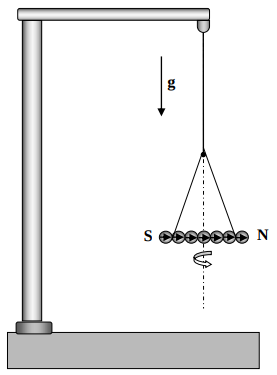
\includegraphics[width=0.5\textwidth]{Images/krut.png}
  \caption{Схема установки для определения горизонтальной составляющей поля Земли.}
\end{figure}

Будем исследовать зависимость периода колебаний от количества шаров в магнитной
стрелке.

Построим график зависимости $T(n)$, аппроксимируем прямой $T=kn$:

\begin{figure}[h]
  \centering
  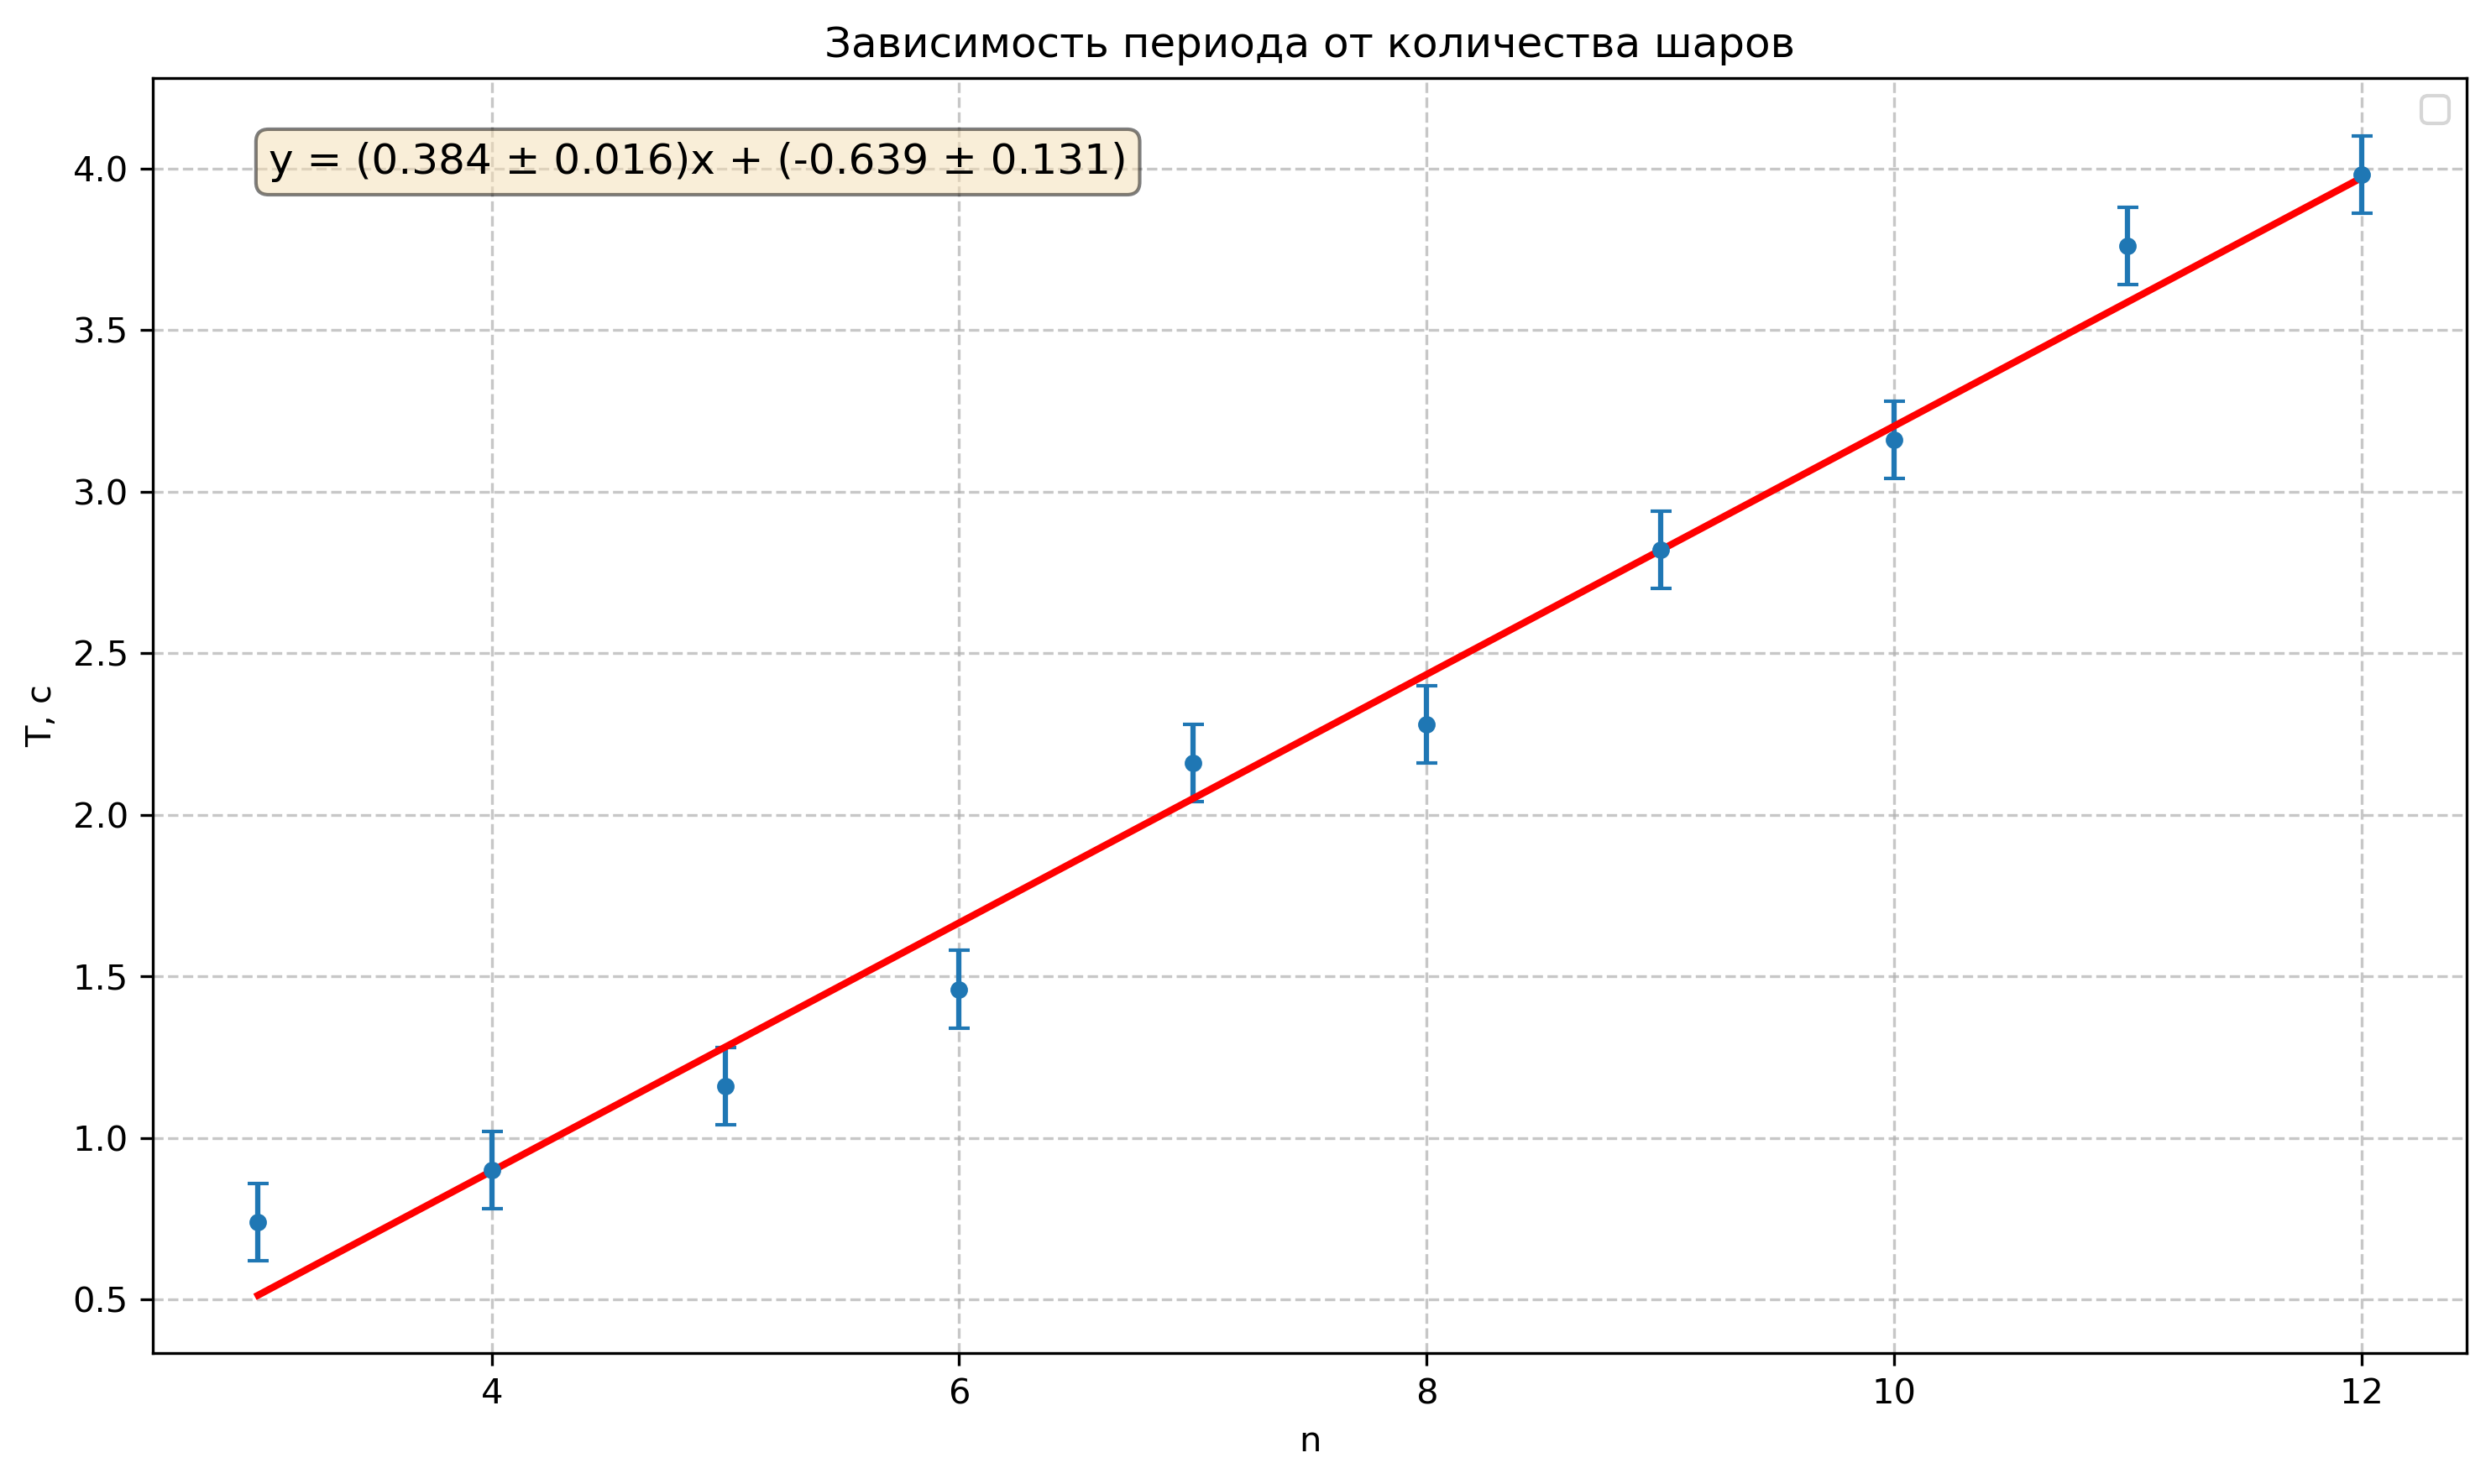
\includegraphics[width=0.9\textwidth]{Images/period.png}
\end{figure}

Из него по формуле $B_h=\pi^2md^2/3k^2P_m$ найдем величину горизонтальной составляющей
магнитного поля.

$k=0.38\pm0.02$

$B_h=0.11\pm0.1\text{Гс}$

Проведем так же эксперимент для замкнутого кольца из шариков: $T=2.4c$

\begin{figure}[h]
  \centering
  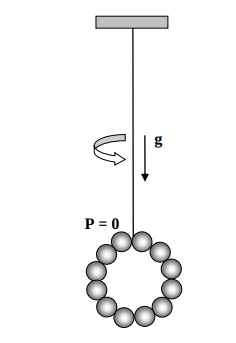
\includegraphics[width=0.2\textwidth]{Images/ring.png}
  \caption{магнитная стрелка, свернутая в кольцо}
\end{figure}

\clearpage
\newpage

\subsection{Определение вертикальной составляющей магнитного поля Земли}

Снова изготовим стрелку из шаров, подвесим ее за середину на нить. С помощью весов
будем определять массу уравновешивающего груза. Таким образом, измерим $M$, действующий
со стороны Земли на стрелку для четных размеров стрелки в шариках.

\begin{figure}[h]
  \centering
  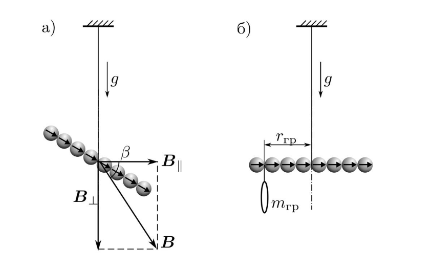
\includegraphics[width=0.5\textwidth]{Images/vert.png}
  \caption{Способ определения момента, действующего со стороны Земли}
\end{figure}

Построим график $M(n)$, аппроксимируем его прямой $M(n)=An$:

\begin{figure}[h]
  \centering
  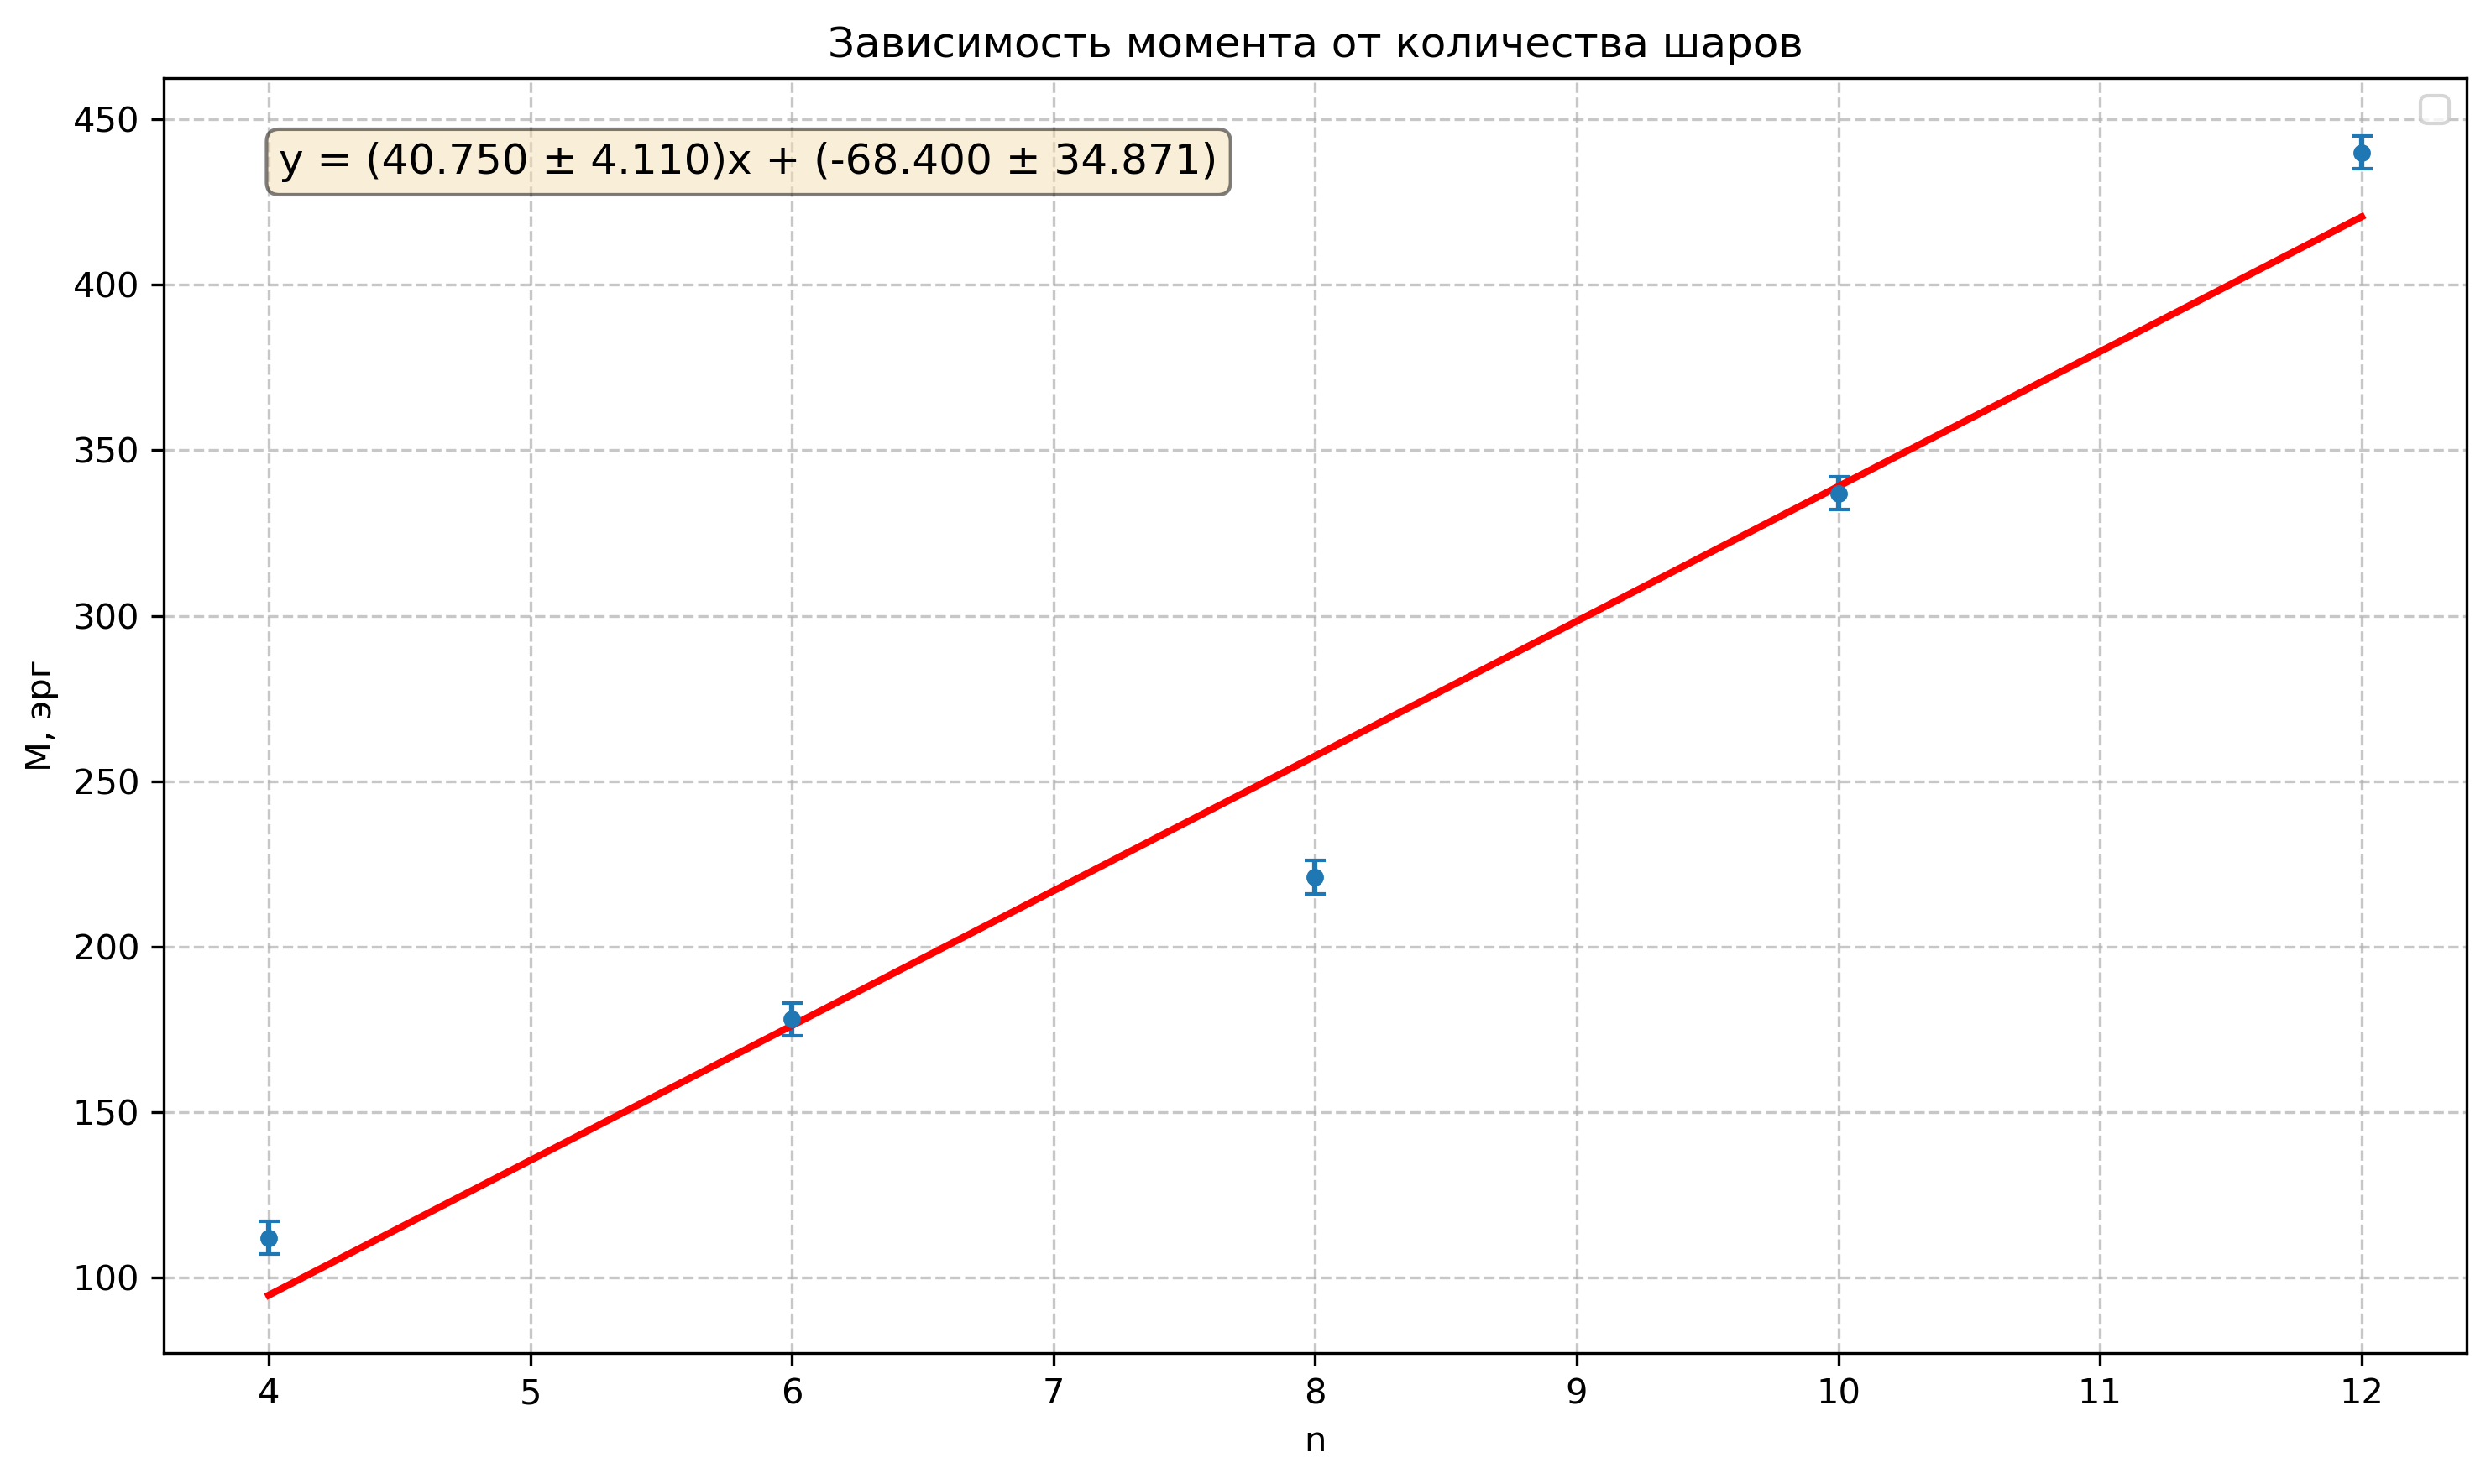
\includegraphics[width=0.9\textwidth]{Images/vertical.png}
\end{figure}

Получаем $B_v=\frac{M}{nm}=(0.37\pm0.3)\text{Гс}$

Сравним значения с табличными: $B_e=0.38\text{Гс}$, $B_t=0.5\text{Гс}$.

\section{3. Выводы}
Получились результаты, отличающиеся от табличных на 1-2 погрешности, поэтому
эксперимент можно считать успешным.

Большую вклад в погрешность измерений второй и третьей части лабораторной
внесла погрешность, возникающая из-за человеческой реакции (при измерении периода с таймером), 
поэтому в третьей части полученное значение поля Земли входит лишь в двойную погрешность
от табличного.


\end{document}
